\documentclass[width=5cm]{standalone}

\usepackage{pgfplots}
\usepgfplotslibrary{colormaps}
\pgfplotsset{compat=newest}

\begin{document}
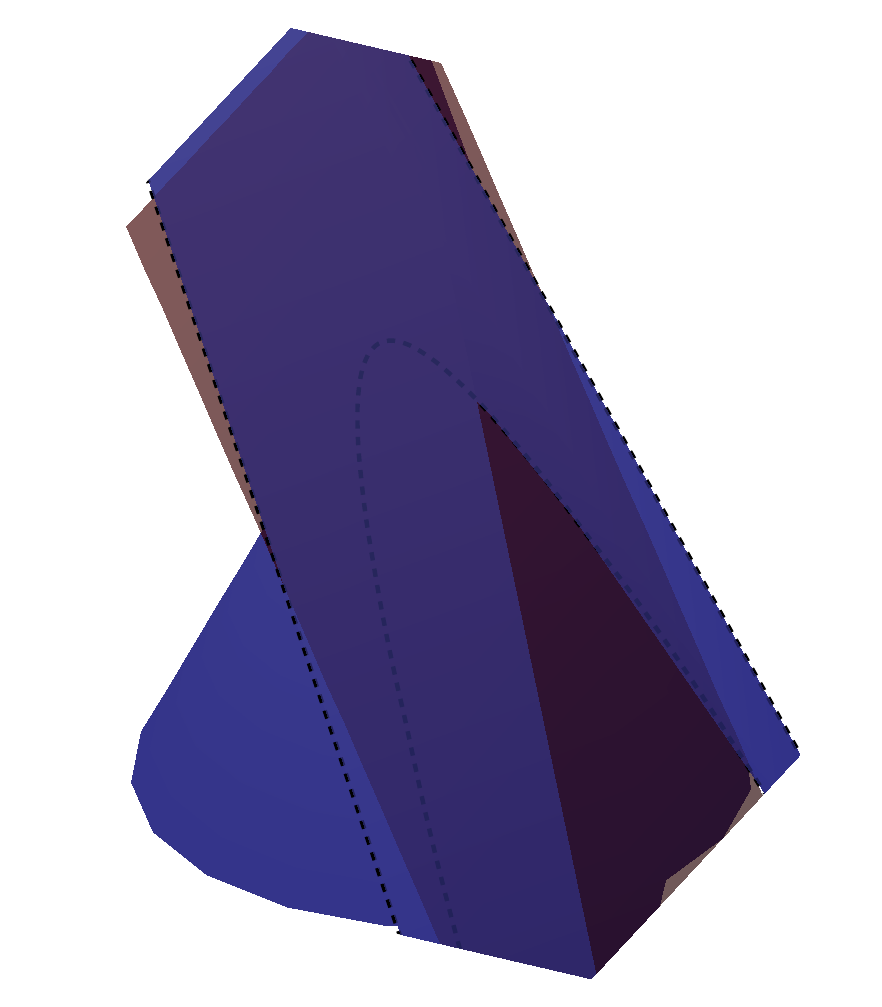
\begin{tikzpicture}
\begin{axis}[
	axis equal image,
	axis line style={draw=none},
	hide axis,
	% grid = both,
	% minor tick num = 2,
	% xlabel = {$x$},
	% ylabel = {$y$},
	% zlabel = {$z$},
	% major grid style = {draw = lightgray},
	% minor grid style = {draw = lightgray!25},
	% legend cell align={left},
	ymin = -1, ymax = 1,
	xmin = -1, xmax = 1,
	scale = 3,
	zmin = 0, zmax = 2,
	z buffer = sort,
]
\pgfmathsetmacro{\th}{25}

\pgfmathsetmacro{\xsamps}{20}
\pgfmathsetmacro{\ysamps}{10}

% bottom of the cone
\addplot3[
	surf,
	shader = interp,
	samples = \xsamps,
	samples y = \ysamps,
	domain = 0:2*pi,
	domain y = 0:1,
	colormap/violet,
]
(
	{cos(deg(x)) + ((sin(\th) /
		(2*sin(\th)-cos(\th)*cos(deg(x))))*cos(deg(x))-cos(deg(x)))*y},
	{sin(deg(x)) + ((sin(\th) /
		(2*sin(\th)-cos(\th)*cos(deg(x))))*sin(deg(x))-sin(deg(x)))*y},
	{0 + (-2*(sin(\th) /
		(2*sin(\th)-cos(\th)*cos(deg(x))))+2-0)*y}
);

% plane
\addplot3[
	surf,
	shader = interp,
	opacity = 0.65,
	domain = -0.65:0.9,
	domain y = -1:1,
	colormap/hot2
] {-cos(\th)/sin(\th)*x+1};

% ellipse
\draw[
	samples = \xsamps,
	smooth,
	domain = 0:2*pi,
	variable = \t,
	dashed,
	ultra thick
]
plot (
	{(sin(\th) /
		(2*sin(\th) - cos(\th)*cos(deg(\t))))*cos(deg(\t))},
	{(sin(\th) /
		(2*sin(\th) - cos(\th)*cos(deg(\t))))*sin(deg(\t))},
	{-2*(sin(\th) /
		(2*sin(\th) - cos(\th)*cos(deg(\t))))+2}
);

% top of the cone
\addplot3[
	surf,
	shader = interp,
	samples = \xsamps,
	samples y = \ysamps,
	domain = 0:2*pi,
	domain y = 0:1,
	opacity = 0.65,
	colormap/violet,
]
(
	{0 + ((sin(\th) /
		(2*sin(\th)-cos(\th)*cos(deg(x))))*cos(deg(x))-0)*y},
	{0 + ((sin(\th) /
		(2*sin(\th)-cos(\th)*cos(deg(x))))*sin(deg(x))-0)*y},
	{2 + (-2*(sin(\th) /
		(2*sin(\th)-cos(\th)*cos(deg(x))))+2-2)*y}
);
\end{axis}
\end{tikzpicture}
\end{document}
